\documentclass[14pt, a4paper, titlepage, fleqn]{extarticle}

\usepackage[russian]{babel}

\usepackage{amsmath}
\usepackage{amssymb}
\usepackage{graphicx}
\usepackage{float}
\usepackage{svg}

\newcommand{\rnc}[1]
    {\MakeUppercase{\romannumeral #1}}
\newcommand{\otv}{\textit{Ответ:} }

\DeclareMathOperator{\D}{\partial}
\DeclareMathOperator{\Ln}{Ln}
\DeclareMathOperator{\Imz}{Im}
\DeclareMathOperator{\Rez}{Re}


\title{Индивидуальное домашнее задание №1 по дисциплине <<Комплексный анализ>>}
\author{Держапольский Юрий Витальевич}
\date{}

\begin{document}

    \maketitle

    \begin{enumerate}
        \item Найти все значения корня: \( \sqrt[4]{-128+ i 128 \sqrt{3}} \).
        \[ 
            \rho = \left\vert -128+ i 128 \sqrt{3} \right\vert 
            = \sqrt{ 2^{7 \cdot 2} + 3 \cdot 2^{7 \cdot 2} } 
            = \sqrt{ 2^2 \cdot 2^{7 \cdot 2} } = 2^8 
        \]
        \[
            \varphi = \pi + \arctg{\frac{128\sqrt{3}}{-128}} = \pi - \arctg{\sqrt{3}} = \frac{2 \pi}{3}
        \]
        \[
            z_k = \sqrt[4]{2^8 \left( \cos{\frac{2 \pi}{3}} + i \sin{\frac{2 \pi}{3}} \right)} =
            4 \left( \cos{\frac{\frac{2 \pi}{3}+2\pi k}{4}} + i \sin{\frac{\frac{2 \pi}{3}+2\pi k}{4}} \right)
            % k = \overline{0,3} 
        \]
        \[
            z_0 = 4 \left( \cos{\frac{\pi}{6}} + i \sin{\frac{\pi}{6}} \right) = 4 \left( \frac{\sqrt{3}}{2} + i \frac{1}{2} \right) = 2\sqrt{3} + 2i
        \]
        \[
            z_1 = 4 \left( \cos{\frac{2\pi}{3}} + i \sin{\frac{2\pi}{3}} \right) = 4 \left( -\frac{1}{2} + i \frac{\sqrt{3}}{2} \right) = -2 + 2\sqrt{3} ~ i
        \]
        \[
            z_2 = 4 \left( \cos{\frac{7\pi}{6}} + i \sin{\frac{7\pi}{6}} \right) = 4 \left( -\frac{\sqrt{3}}{2} - i \frac{1}{2} \right) = -2\sqrt{3} - 2i
        \]
        \[
            z_3 = 4 \left( \cos{\frac{5\pi}{3}} + i \sin{\frac{5\pi}{3}} \right) = 4 \left( \frac{1}{2} - i \frac{\sqrt{3}}{2} \right) = 2 - 2\sqrt{3} ~ i
        \]

        \otv \(
            \displaystyle
            \sqrt[4]{-128+ i 128 \sqrt{3}} = 
            \left\lbrace
            \begin{aligned}
                2\sqrt{3} + 2i \\
                -2 + 2\sqrt{3} ~ i \\
                -2\sqrt{3} - 2i \\
                2 - 2\sqrt{3} ~ i
            \end{aligned}
            \right.
        \)

        \pagebreak

        \item Представить в алгебраической форме: \( \sh{\left( 1 + 4 \pi i \right)} \).
        \[
            \sh{\left( 1 + 4 \pi i \right)} = \sh{1} \cdot \ch{4 \pi i} + \ch{1} \cdot \sh{4 \pi i} =
        \]
        \[
             = \sh{1} \cdot \cos{4 \pi} + \ch{1} \cdot i \sin{4 \pi} = \sh{1}
        \]

        \otv \( \sh{\left( 1 + 4 \pi i \right)} = \sh 1 \)
        
        \item Представить в алгебраической форме: \( \displaystyle \arctg{\left( \frac{-2\sqrt{3} + 3i}{7} \right)} \).
        
        Обозначим искомое как \( z \), и \( \displaystyle \omega = \frac{-2\sqrt{3} + 3i}{7} \). 
        Тогда \( \tg z = \omega \). Отсюда получаем:
        \( 
            \displaystyle
            z = - \frac{i}{2} \Ln \left( \frac{1 + i \omega}{1 - i \omega} \right)
        \).
        \[
            \zeta = \frac{1 + i \omega}{1 - i \omega} = \frac{7 - 2\sqrt{3} ~ i - 3}{7 + 2\sqrt{3} ~ i + 3} =
            \frac{4 - 2\sqrt{3} ~ i}{10 + 2\sqrt{3} ~ i} \cdot \frac{10 - 2\sqrt{3} ~ i}{10 - 2\sqrt{3} ~ i} =
        \]
        \[
            = \frac{28 - 28 \sqrt{3} ~ i}{112}= \frac{1 - \sqrt{3} ~ i}{4}
        \]
        \[
            |\zeta| = \sqrt{ \frac{1}{16} + \frac{3}{16} } = \frac{1}{2}; \quad
            \arg{\zeta} = -\frac{\pi}{3}
        \]

        \[
            z = -\frac{i}{2} \Ln \left( \zeta \right) = -\frac{i}{2} \left( \ln |\zeta| + i (\arg \zeta + 2 \pi n) \right) =
        \]
        \[
            = -\frac{i}{2} \left( -\ln 2 + i \left( -\frac{\pi}{3} + 2 \pi n \right) \right) = \pi n - \frac{\pi}{6} + \frac{i \ln 2}{2}, n \in \mathbb{Z}
        \]

        \otv \( \displaystyle \arctg{\left( \frac{-2\sqrt{3} + 3i}{7} \right)} = \pi n - \frac{\pi}{6} + \frac{i \ln 2}{2}, n \in \mathbb{Z} \)

        \pagebreak

        \item Представить в алгебраической форме: \( (-i)^{5i} \).
        \[
            (-i)^{5i} = \left( e^{i(-\pi/2 + 2 \pi n)} \right)^{5i} = e^{5\pi/2 + 10\pi n}, ~ n \in \mathbb{Z}
        \]

        \otv \( (-i)^{5i} = e^{5\pi/2 + 10\pi n}, ~ n \in \mathbb{Z} \)

        \item Представить в алгебраической форме: \( \Ln\left( e^2 \right) \).
        \[
            \Ln\left( e^2 \right) = \ln \left\vert e^2 \right\vert + i \left(\arg \left(e^2\right) + 2 \pi n\right) = 2 + 2 \pi n i, ~ n \in \mathbb{Z}
        \]

        \otv \( \Ln\left( e^2 \right) = 2 + 2 \pi n i, ~ n \in \mathbb{Z} \)

        \item Вычертить область, заданную неравенствами: \\
        \( D = \left\lbrace z: ~ |z - 1 - i| \leq 1, ~ \Imz z > 1, ~ \Rez z \geq 1 \right\rbrace \).

        \begin{figure}[H]
            \centering
            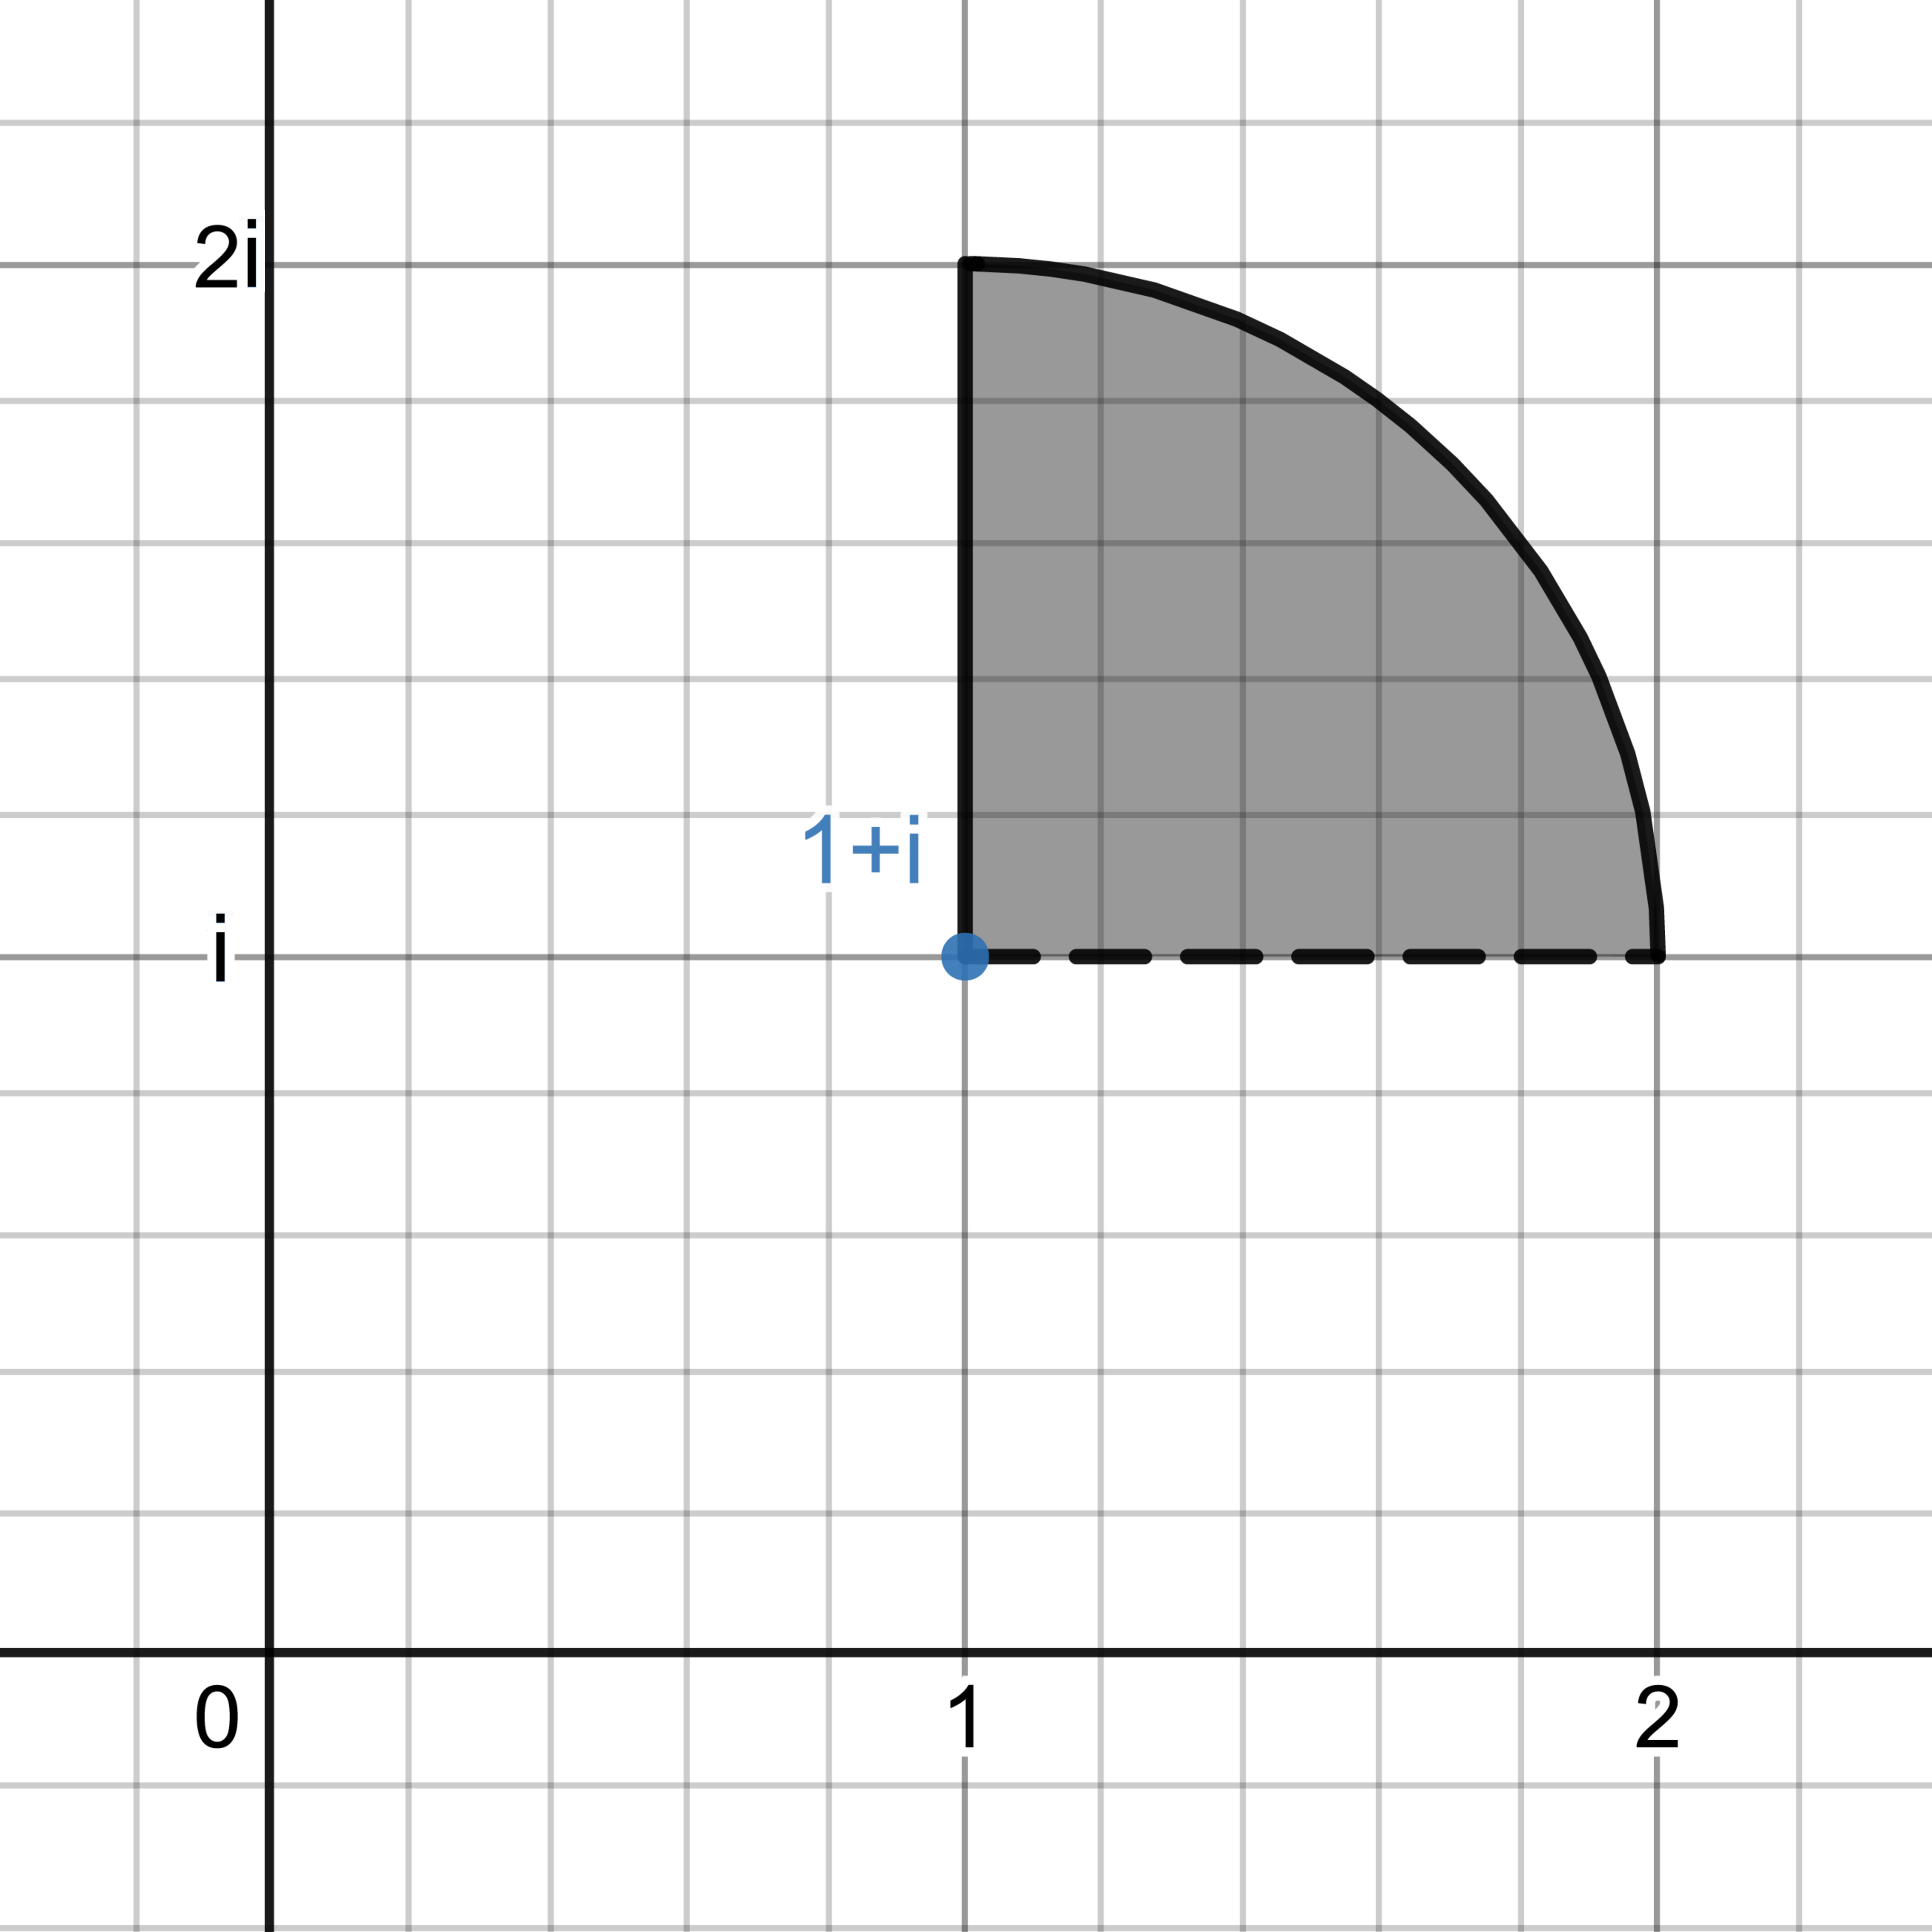
\includegraphics[width=8cm]{pictures/c_idz1_6.pdf}
        \end{figure}

        \pagebreak

        \item Определить вид пути и в случае, когда он проходит через точку \( \infty \), исследовать
        его поведение в этой точке. \( z = -\sec t + i3 \tg t \).

        Наименьший период функций \( \tg t \) и \( \sec t \) равен 2 \(\pi\),
        поэтому достаточно построить кривую для \( \displaystyle t \in \left( -\frac{\pi}{2}; \frac{\pi}{2} \right) \cup \left( \frac{\pi}{2}; \frac{3\pi}{2} \right) \).
        \[
            \left\lbrace
            \begin{aligned}
                x &= -\sec t \\
                y &= 3 \tg t
            \end{aligned}
            \right. \quad
            \left\lbrace
            \begin{aligned}
                x^2 &= \sec^2 t = 1 + \tg^2 t\\
                y^2 &= 9 \tg^2 t
            \end{aligned}
            \right. \implies 
            x^2 = 1 + \frac{y^2}{9}
        \]

        \( \displaystyle x^2 - \frac{y^2}{9} = 1 \) -- каноническое уравнение гиперболы.
        \( \displaystyle x \pm \frac{y}{3} = 0 \) -- асимптоты.

        \begin{figure}[H]
            \centering
            \includegraphics[width=8cm]{pictures/c_idz1_7.pdf}
        \end{figure}
        
        При \( t \to -\frac{\pi}{2} + 0, x \to -\infty, y \to -\infty \).

        При \( t \to \frac{\pi}{2} - 0, x \to -\infty, y \to +\infty \).

        При \( t \to \frac{\pi}{2} + 0, x \to +\infty, y \to -\infty \).

        При \( t \to \frac{3\pi}{2} - 0, x \to +\infty, y \to +\infty \).

        \pagebreak

        \item Восстановить голоморфную в окрестности точки \( z_0 \) функцию \( f(z) \) по известной
        мнимой части \( v(x,y) \) и начальному значению \( f(z_0) \): 
        \( 
            \displaystyle
            v = \frac{e^{2x}-1}{e^x}\sin{y}, \quad f(0) = 2
        \).
        \[ v = \left( e^x - e^{-x} \right) \sin y \]
        Проверка:
        \[
            \begin{matrix}
                \frac{\D v}{\D x} = \left( e^{x} + e^{-x} \right) \sin y &&
                \frac{\D v}{\D y} = \left( e^{x} - e^{-x} \right) \cos y \\
                \frac{\D^2 v}{\D x^2} = \left( e^{x} - e^{-x} \right) \sin y && 
                \frac{\D^2 v}{\D y^2} = -\left( e^{x} - e^{-x} \right) \sin y
            \end{matrix}
        \]
        \[
            \frac{\D^2 v}{\D x^2} + \frac{\D^2 v}{\D y^2} = 0
        \]
        Функция удовлетворяет условию Лапласа. 
        \[
            \left\lbrace
            \begin{aligned}
                &\frac{\D u}{\D x} = \frac{\D v}{\D y} = \left( e^{x} - e^{-x} \right) \cos y \\
                &\frac{\D u}{\D y} = -\frac{\D v}{\D x} = - \left( e^{x} + e^{-x} \right) \sin y
            \end{aligned}   
            \right.
        \]
        \[
            \left\lbrace
            \begin{aligned}
                &u = \left( e^{x} + e^{-x} \right) \cos y + C_1(y) \\
                &u = \left( e^{x} + e^{-x} \right) \cos y + C_2(x)
            \end{aligned}   
            \right.
        \]
        \[
            u = \left( e^{x} + e^{-x} \right) \cos y + C
        \]

        \[
            f(x,y) = u(x,y) + i v(x,y) = \left( e^{x} + e^{-x} \right) \cos y + C + i \left( e^x - e^{-x} \right) \sin y =
        \]
        \[
            =  \left( e^{x} + e^{-x} \right) \frac{e^{iy} + e^{-iy}}{2} + i \left( e^x - e^{-x} \right) \frac{e^{iy} - e^{-iy}}{2i} + C =
        \]
        \[
            = \frac{e^{x+iy} +e^{x-iy} + e^{-x+iy} + e^{-x-iy} + e^{x+iy} -e^{x-iy} - e^{-x+iy} + e^{-x-iy} }{2} + C =
        \]
        \[
            = e^{x+iy} + e^{-x-iy} + C = e^z + e^{-z} + C
        \]
        \[
            f(0) = 1 + 1 + C = 2 \implies C = 0
        \]
        \otv \( f(z) = e^z + e^{-z} \)

        \item Вычислить интеграл от функции комплексной переменной по данному пути
        \( \int_{ABC} \left( z^2 + \cos z \right) ~ dz \); ABC - ломаная, 
        \( z_A = 0, z_B = 1, z_C = i \). 
        \[
            \int_{ABC} \left( z^2 + \cos z \right) ~ dz = \int_{0}^{i} \left( \frac{z^3}{3} + \sin z \right)' ~ dz = 
            \left( \frac{z^3}{3} + \sin z \right) \bigg\vert_0^i = 
        \]
        \[
            = -\frac{i}{3} + \sin i - 0 = i \left( \sh{1} -\frac{1}{3} \right)
        \]

        \otv \( \int_{ABC} \left( z^2 + \cos z \right) ~ dz = i \left( \sh{1} -\frac{1}{3} \right) \).

        \item Найти радиус сходимости степенного ряда: \(  \sum_{n=1}^{\infty} \left( n + i \right)^2 \cdot z^{n^2} \).
        \[
            C_k = \left\lbrace
            \begin{matrix}
                (n + i)^2, && k = n^2 \\
                0, && k \neq n^2
            \end{matrix}
            \right.
        \]
        \[
            \left| C_{n^2} \right| = \left| (n+i)^2 \right| = \left| n^2 - 1 + 2ni \right| = \sqrt{ \left( n^2-1 \right)^2 + (2n)^2 } =
        \]
        \[
            = \sqrt{n^4 - 2n^2 + 1 + 4n^2} = \sqrt{ \left( n^2 + 1 \right)^2 } = n^2 + 1
        \]
        \[
            \sqrt[n^2]{\left| C_{n^2} \right|} = \sqrt[n^2]{ n^2 + 1 } \xrightarrow{n\to\infty} 1
        \]

        \otv \( R = 1 \) и область сходимости -- круг \( |z| < 1 \).

        \item Найти все лорановкие разложения данной функции в \( 0 \) и в \( \infty \): \( \displaystyle f(z) = \frac{z-4}{z^4+z^3-2z^2} \).
        
        Разложим в точке \( 0 \):
        \[
            f(z) = \frac{z-4}{z^4+z^3-2z^2} = \frac{2}{z^2} + \frac{1}{2 z} + \frac{1}{2 (z + 2)} - \frac{1}{z - 1} =
        \]
        \[
            = \frac{2}{z^2} + \frac{1}{2 z} + \frac{1}{4} \frac{1}{(1 + z/2)} + \frac{1}{1 - z} =
        \]
        \[
            = \frac{2}{z^2} + \frac{1}{2 z} + \frac{1}{4} \sum_{n=0}^\infty (-1)^n \frac{z^n}{2^n} + \sum_{n=0}^\infty z^n
             = \frac{2}{z^2} + \frac{1}{2 z} + \sum_{n=0}^\infty \left(1 + \frac{(-1)^n}{2^{n+2}} \right) z^n
        \]
        \[
            C_n = \left\lbrace
                \begin{aligned}
                    &0, \quad n \leq -3, \\
                    &2, \quad n = -2 \\
                    &\frac{1}{2}, \quad n = -1 \\
                    &1 + \frac{(-1)^n}{2^{n+2}}, \quad n \geq 0
                \end{aligned}
            \right.
        \]

        % Разложим в точке \( \infty \):
        % \[
        %     f(z) = \frac{2}{z^2} + \frac{1}{2 z} + \frac{1}{4} \frac{1}{(1 + z/2)} + \frac{1}{1 - z} =
        %     \frac{2}{z^2} + \frac{1}{2 z} + \frac{1}{2z} \frac{1}{(1 + 2/z)} - \frac{1}{z} \frac{1}{1 - 1/z} =
        % \]
        % \[
        %     = \frac{2}{z^2} + \frac{1}{2 z} + \frac{1}{2z} \sum_{n=0}^\infty (-1)^n \frac{2^n}{z^n} - \frac{1}{z} \sum_{n=0}^\infty \frac{1}{z^n} 
        %     = \frac{2}{z^2} + \frac{1}{2 z} + \sum_{n=0}^\infty (-1)^n \frac{2^{n-1}}{z^{n+1}} - \sum_{n=0}^\infty \frac{1}{z^{n+1}} =
        % \]
        % \[
        %     = \frac{2}{z^2} + \frac{1}{2 z} + \sum_{n'=-\infty}^{-1} (-1)^{n'+1} \frac{z^{n'} }{2^{n'+2}} - \sum_{n=-\infty}^{-1} z^n
        %     = \frac{2}{z^2} + \frac{1}{2 z} + \sum_{n=-\infty}^{-1} \left( \frac{(-1)^{n+1}}{2^{n+2}} - 1 \right) z^n =
        % \]
        % \[
        %     = \sum_{n=-\infty}^{-3} \left( \frac{(-1)^{n+1}}{2^{n+2}} - 1 \right) z^n
        % \]
        % \[
        %     C_n = \left\lbrace
        %         \begin{aligned}
        %             &\frac{(-1)^{n+1}}{2^{n+2}} - 1, \quad n \leq -3 \\
        %             &0, \quad n \geq -2
        %         \end{aligned}
        %     \right.
        % \]

        Разложим в точке \( z = \infty \). Заменим \( z = \frac{1}{w} \), значит раскладываем в точке \( w = 0 \):
        \[
            f(w) = \frac{\frac{1}{w}-4}{\frac{1}{w^4} + \frac{1}{w^3}-\frac{2}{w^2}} = \frac{w^3-4w^4}{1+w-2w^2} = 
        \]
        \[
            = 2w^2 + \frac{w}{2} - \frac{1}{1-w} - \frac{1}{4(1+2w)} + \frac{5}{4} =
        \]
        \[
            = 2w^2 + \frac{w}{2} + \frac{5}{4} - \sum_{n=0}^{\infty} w^n - \frac{1}{4} \sum_{n=0}^{\infty} (-1)^n (2w)^n =
        \]
        \[
            = 2w^2 + \frac{w}{2} + \frac{5}{4} - \sum_{n=0}^{\infty} \left(1 + \frac{(-2)^n}{4} \right) w^n =
        \]
        \[
            = \frac{5}{4} - \frac{5}{4} + \frac{w}{2} - \frac{w}{2} + 2w^2 - 2w^2 - \sum_{n=3}^{\infty} \left(1 + \frac{(-2)^n}{4} \right) w^n =
        \]
        \[
            = - \sum_{n=3}^{\infty} \left(1 + \frac{(-2)^n}{4} \right) w^n 
        \]
        Сделаем обратную замену:
        \[
            - \sum_{n=3}^{\infty} \left(1 + \frac{(-2)^n}{4} \right) \frac{1}{z^n} = - \sum_{n=-\infty}^{-3} \left(1 + \frac{(-1)^n}{4 \cdot 2^n} \right) z^n = \sum_{n=-\infty}^{-3} \left(\frac{(-1)^{n+1}}{2^{n+2}} - 1 \right) z^n
        \]
        \[
            C_n = \left\lbrace
                \begin{aligned}
                    &\frac{(-1)^{n+1}}{2^{n+2}} - 1, \quad n \leq -3 \\
                    &0, \quad n \geq -2
                \end{aligned}
            \right.
        \]

        
        \item Найти все лорановские разложения функции по степеням \( z - z_0 \): \( \displaystyle f(z) = \frac{z-2}{(z+1)(z-3)}, \quad z_0 = 3+i \).  
        
        \[
            f(z) = \frac{z-2}{(z+1)(z-3)} = \frac{3}{4} \cdot \frac{1}{z+1} + \frac{1}{4} \cdot \frac{1}{z-3}
        \]

        Функция голоморфна в 3-х кольцах:
        \[
            \begin{aligned}
                K_1:&~ 0<|z-z_0|<1 \\
                K_2:&~ 1 < |z-z_0|<\sqrt{17} \\
                K_3:&~ \sqrt{17}<|z-z_0|<\infty
            \end{aligned}
        \]
        
        Разложим в \( K_1 \):
        \[
            \frac{1}{z+1} = \frac{1}{z - z_0 + z_0+1 } = \frac{1}{z_0+1} \cdot \frac{1}{1+\frac{z-z_0}{z_0+1}} =
        \]
        \[
            = \frac{1}{z_0+1} \sum_{n=0}^{\infty} (-1)^n \left(\frac{z-z_0}{z_0+1} \right)^n = \sum_{n=0}^{\infty} \frac{ (-1)^n }{(z_0+1)^{n+1}} (z-z_0)^n
        \]
        \[
            \frac{1}{z-3} = \frac{1}{z- z_0 + z_0 - 3} = \frac{1}{z_0-3} \cdot \frac{1}{1+\frac{z-z_0}{z_0-3}} =
        \]
        \[
            = \frac{1}{z_0-3} \sum_{n=0}^{\infty} (-1)^n \left( \frac{z-z_0}{z_0-3} \right)^n = \sum_{n=0}^{\infty} \frac{(-1)^n}{(z_0-3)^{n+1}} (z-z_0)^n
        \]
        \[
            f(z) = \sum_{n=0}^{\infty} \frac{ 3(-1)^n }{4(z_0+1)^{n+1}} (z-z_0)^n + \sum_{n=0}^{\infty} \frac{(-1)^n}{4(z_0-3)^{n+1}} (z-z_0)^n =
        \]
        \[
            = \sum_{n=0}^{\infty} \frac{(-1)^n}{4} \left( \frac{3}{(z_0+1)^{n+1}} + \frac{1}{(z_0-3)^{n+1}} \right) (z-z_0)^n
        \]

        \pagebreak

        Разложим в \( K_2 \):

        \( \displaystyle \frac{1}{z+1} \) аналогично разложению в \( K_1 \).
        \[
            \frac{1}{z-3} = \frac{1}{z- z_0 + z_0 - 3} = \frac{1}{z-z_0} \cdot \frac{1}{1 + \frac{z_0-3}{z-z_0}} =
        \]
        \[
            = \frac{1}{z-z_0} \sum_{n=0}^{\infty} (-1)^n \left( \frac{z_0-3}{z-z_0} \right)^n = \sum_{n=0}^{\infty} (-1)^n \frac{(z_0-3)^n}{(z-z_0)^{n+1}} =
        \]
        \[
            = \sum_{n=-\infty}^{-1} (-1)^{n+1} \frac{(z-z_0)^n}{(z_0-3)^{n+1}}
        \]
        \[
            f(z) = \sum_{n=0}^{\infty} \frac{ 3(-1)^n }{4(z_0+1)^{n+1}} (z-z_0)^n + \sum_{n=-\infty}^{-1} \frac{(-1)^{n+1}}{4(z_0-3)^{n+1}} (z-z_0)^n
        \]

        Разложим в \( K_3 \): 
        \[
            \frac{1}{z+1} = \frac{1}{z-z_0+z_0+1} = \frac{1}{z-z_0} \cdot \frac{1}{1+\frac{z_0+1}{z-z_0}} =
        \]
        \[
            = \frac{1}{z-z_0} \sum_{n=0}^{\infty} (-1)^n \left( \frac{z_0+1}{z-z_0} \right)^n = \sum_{n=0}^{\infty} (-1)^n \frac{(z_0+1)^n}{(z-z_0)^{n+1}} =
        \]
        \[
            = \sum_{n=-\infty}^{-1} \frac{(-1)^{n+1}}{(z_0+1)^{n+1}} (z-z_0)^n
        \]
        \( \displaystyle \frac{1}{z-3} \) аналогично разложению в \( K_2 \). 
        \[
            f(z) = \sum_{n=-\infty}^{-1} \frac{3(-1)^{n+1}}{4(z_0+1)^{n+1}} (z-z_0)^n + \sum_{n=-\infty}^{-1} \frac{(-1)^{n+1}}{4(z_0-3)^{n+1}} (z-z_0)^n =
        \]
        \[
            = \sum_{n=-\infty}^{-1} \frac{(-1)^{n+1}}{4} \left( \frac{3}{(z_0+1)^{n+1}} + \frac{1}{(z_0-3)^{n+1}}\right) (z-z_0)^n
        \]

        
        \pagebreak

        \item Данную функцию разложить в ряд Лорана в окрестности точки \( z_0 \): \( \displaystyle f(z) = \cos \frac{3z}{z-i}, z_0 = i \).
        \[
            f(z) = \cos \frac{3z}{z-i} = \cos \left( 3 + \frac{3i}{z-i} \right) = \cos 3 \cdot \cos \frac{3i}{z-i} - \sin 3 \cdot \sin \frac{3i}{z-i} =
        \]
        \[
            = \cos 3 \cdot \sum_{n=0}^{\infty} \frac{(-1)^n}{(2n)!} \left( \frac{3i}{z-i} \right)^{2n}  - \sin 3 \cdot \sum_{n=0}^{\infty} \frac{(-1)^n}{(2n+1)!} \left( \frac{3i}{z-i} \right)^{2n+1} =
        \]
        \[
            = \sum_{n=-\infty}^{0} \frac{(-1)^n \cos 3}{(-2n)! (3i)^{2n}} \left( z-i \right)^{2n}  - \sum_{n=-\infty}^{0} \frac{(-1)^n \sin 3}{(1-2n)! (3i)^{2n-1}} \left( z-i \right)^{2n-1}
        \]
        \[
            C_k = \left\lbrace
                \begin{aligned}
                    &\frac{(-1)^n \cos 3}{(-2n)! (3i)^{2n}}, \quad k = 2n, ~ n \leq 0, \\
                    &\frac{(-1)^n \sin 3}{(1-2n)! (3i)^{2n-1}}, \quad k = 2n-1, ~ n \leq 0, \\
                    &0, \quad k \geq 1
                \end{aligned}
            \right.
        \]  

        \item Определить тип особой точки \( z = 0 \) для данной функции: \( \displaystyle f(z) = \frac{\cos 5z -1 }{\ch z - 1 - z^2/2} \).
        \[
            \lim\limits_{z\to 0} f(z) = \lim\limits_{z\to 0} \frac{\cos 5z -1 }{\ch z - 1 - z^2/2} =
            \lim\limits_{z\to 0} \frac{1 - \frac{(5z)^2}{2!} + \frac{(5z)^4}{4!} + o(z^5) -1 }{1 + \frac{z^2}{2!} + \frac{z^4}{4!} + o(z^5) - 1 - z^2/2} =
        \]
        \[
            = \lim\limits_{z\to 0} \frac{-\frac{(5z)^2}{2!} + \frac{(5z)^4}{4!} + o(z^5)}{\frac{z^4}{4!} + o(z^5)} = 
            \lim\limits_{z\to 0} \frac{z^2}{z^4} \frac{-\frac{5^2}{2!} + \frac{5^4 z^2}{4!} + o(z^3)}{\frac{1}{4!} + o(z)} = 
            \lim\limits_{z\to 0} \frac{1}{z^2} \frac{-\frac{5^2}{2!}}{\frac{1}{4!}} = \infty
        \]
        \[
            \lim\limits_{z\to 0} \left( z^2 \cdot f(z) \right) = \frac{-\frac{5^2}{2!}}{\frac{1}{4!}}
        \]
        \otv \( z = 0 \) для \( f(z) \) является полюсом 2-го порядка.

        \item Для данной функции найти все изолированные особые точки и определить их тип: \( \displaystyle f(z) = \frac{z^2+1}{(z-i)^2(z^2+4)} \).
        \[
            f(z) = \frac{(z+i)(z-i)}{(z-i)^2(z+2i)(z-2i)} = \frac{(z+i)}{(z-i)(z+2i)(z-2i)}
        \]
        Особые точки: \( z_1 = i, z_2 = 2i, z_3 = -2i, z_4 = \infty \).
        \begin{enumerate}
            \item \( \lim\limits_{z\to i} f(z) = \infty \implies z_0 \) -- полюс 1-го порядка. 
            \item \( \lim\limits_{z\to 2i} f(z) = \infty \implies z_1 \) -- полюс 1-го порядка. 
            \item \( \lim\limits_{z\to -2i} f(z) = \infty \implies z_2 \) -- полюс 1-го порядка.
            \item \( \lim\limits_{z\to \infty} f(z) = 0 \implies z_3 \) -- устранимая особая точка. 
        \end{enumerate}
    \end{enumerate}




\end{document}